% Copyright 2006 by Till Tantau
%
% This file may be distributed and/or modified
%
% 1. under the LaTeX Project Public License and/or
% 2. under the GNU Free Documentation License.
%
% See the file doc/generic/pgf/licenses/LICENSE for more details.

\section{Tutorial: A Picture for Karl's Students}

This tutorial is intended for new users of \tikzname. It
does not give an exhaustive account of all the features of \tikzname,
just of those that you are likely to use right away. 

Karl is a math and chemistry high-school teacher. He used to create
the graphics in his worksheets and exams using \LaTeX's |{picture}|
environment. While the results were acceptable, creating the graphics
often turned out to be a lengthy process. Also, there tended to be
problems with lines having slightly wrong angles and circles also
seemed to be hard to get right. Naturally, his students could not care
less whether the lines had the exact right angles and they find
Karl's exams too difficult no matter how nicely they were drawn. But
Karl was never entirely satisfied with the result.

Karl's son, who was even less satisfied with the results (he did not
have to take the exams, after all),  told Karl that he might wish
to try out a new package for creating graphics. A bit confusingly,
this package seems to have two names: First, Karl had to download and
install a package called \pgfname. Then it turns out that inside this
package there is another package called \tikzname, which is supposed to
stand for ``\tikzname\ ist \emph{kein}  Zeichenprogramm.'' Karl finds this
all a bit strange and \tikzname\ seems to indicate that the package
does not do what he needs. However, having used \textsc{gnu}
software for quite some time and ``\textsc{gnu} not being Unix,''
there seems to be hope yet. His son assures him that \tikzname's name is
intended to warn people that \tikzname\ is not a program that you can
use to draw graphics with your mouse or tablet. Rather, it is more
like a ``graphics language.''


\subsection{Problem Statement}

Karl wants to put a graphic on the next worksheet for his
students. He is currently teaching his students about sine and
cosine. What he would like to have is something that looks like this
(ideally):

\noindent
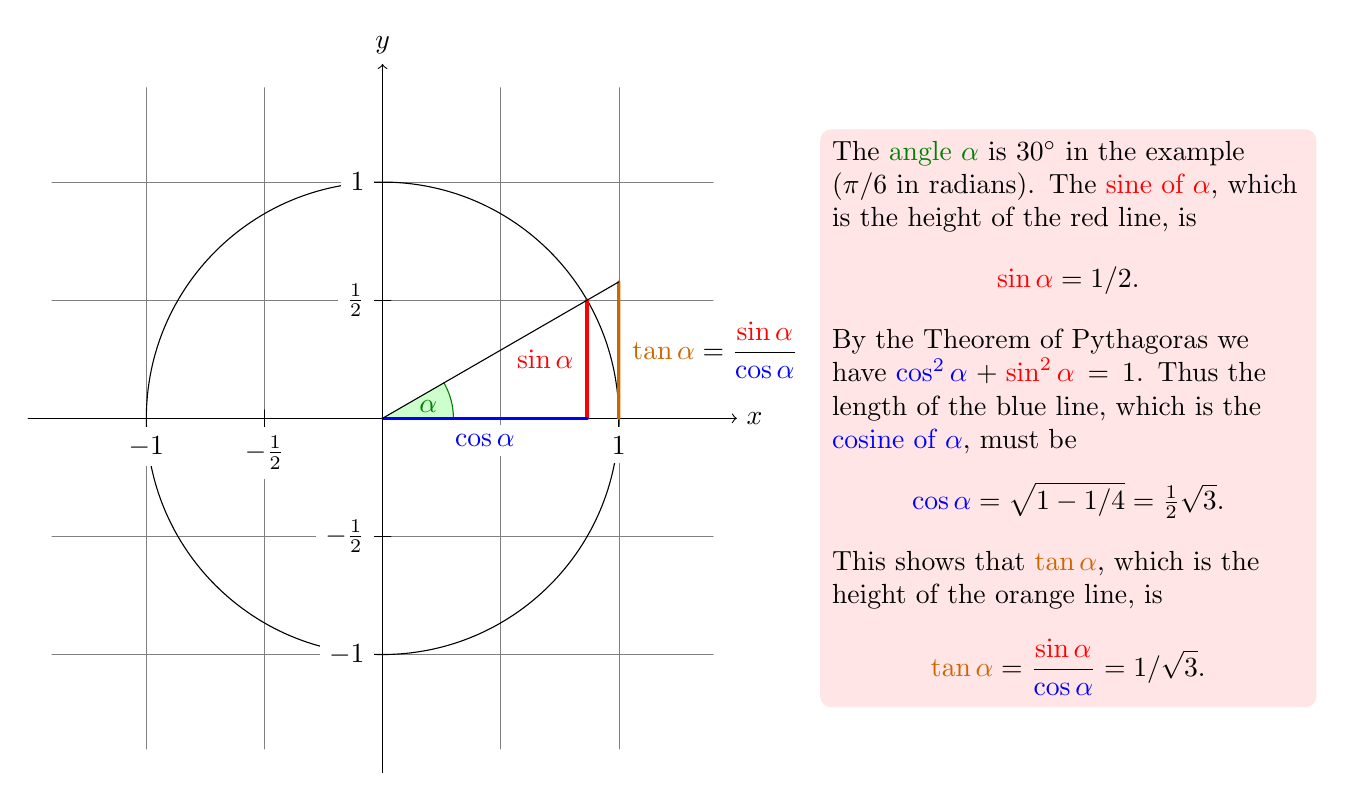
\begin{tikzpicture}
  [scale=3,line cap=round,
   % Styles
   axes/.style=,
   important line/.style={very thick},
   information text/.style={rounded corners,fill=red!10,inner sep=1ex}]

  % Local definitions
  \def\costhirty{0.8660256}

  % Colors
  \colorlet{anglecolor}{green!50!black}
  \colorlet{sincolor}{red}
  \colorlet{tancolor}{orange!80!black}
  \colorlet{coscolor}{blue}

  % The graphic
  \draw[help lines,step=0.5cm] (-1.4,-1.4) grid (1.4,1.4);

  \draw (0,0) circle [radius=1cm];

  \begin{scope}[axes]
    \draw[->] (-1.5,0) -- (1.5,0) node[right] {$x$};
    \draw[->] (0,-1.5) -- (0,1.5) node[above] {$y$};

    \foreach \x/\xtext in {-1, -.5/-\frac{1}{2}, 1}
      \draw[xshift=\x cm] (0pt,1pt) -- (0pt,-1pt) node[below,fill=white] {$\xtext$};

    \foreach \y/\ytext in {-1, -.5/-\frac{1}{2}, .5/\frac{1}{2}, 1}
      \draw[yshift=\y cm] (1pt,0pt) -- (-1pt,0pt) node[left,fill=white] {$\ytext$};
  \end{scope}

  \filldraw[fill=green!20,draw=anglecolor] (0,0) -- (3mm,0pt) arc(0:30:3mm);
  \draw (15:2mm) node[anglecolor] {$\alpha$};

  \draw[important line,sincolor]
    (30:1cm) -- node[left=1pt,fill=white] {$\sin \alpha$} +(0,-.5);

  \draw[important line,coscolor]
    (0,0) -- node[below=2pt,fill=white] {$\cos \alpha$} (\costhirty,0);

  \draw[important line,tancolor] (1,0) --
    node [right=1pt,fill=white]
    {
      $\displaystyle \tan \alpha \color{black}=
      \frac{{\color{sincolor}\sin \alpha}}{\color{coscolor}\cos \alpha}$
    } (intersection of 0,0--30:1cm and 1,0--1,1) coordinate (t);

  \draw (0,0) -- (t);

  \draw[xshift=1.85cm] node [right,text width=6cm,information text]
    {
      The {\color{anglecolor} angle $\alpha$} is $30^\circ$ in the
      example ($\pi/6$ in radians). The {\color{sincolor}sine of
        $\alpha$}, which is the height of the red line, is
      \[
      {\color{sincolor} \sin \alpha} = 1/2.
      \]
      By the Theorem of Pythagoras we have ${\color{coscolor}\cos^2 \alpha} +
      {\color{sincolor}\sin^2\alpha} =1$. Thus the length of the blue
      line, which is the {\color{coscolor}cosine of $\alpha$}, must be
      \[
      {\color{coscolor}\cos\alpha} = \sqrt{1 - 1/4} = \textstyle
      \frac{1}{2} \sqrt 3.
      \]%
      This shows that {\color{tancolor}$\tan \alpha$}, which is the
      height of the orange line, is
      \[
      {\color{tancolor}\tan\alpha} = \frac{{\color{sincolor}\sin
          \alpha}}{\color{coscolor}\cos \alpha} = 1/\sqrt 3.
      \]%
    };
\end{tikzpicture}


\subsection{Setting up the Environment}

In \tikzname, to draw a picture, at the start of the picture
you need to tell \TeX\ or \LaTeX\ that you want to start a picture. In
\LaTeX\ this is done using the environment |{tikzpicture}|, in plain
\TeX\ you just use |\tikzpicture| to start the picture and
|\endtikzpicture| to end it.

\subsubsection{Setting up the Environment in \LaTeX}

Karl, being a \LaTeX\ user, thus sets up his file as follows:

\begin{codeexample}[code only]
\documentclass{article} % say
\usepackage{tikz}
\begin{document}
We are working on
\begin{tikzpicture}
  \draw (-1.5,0) -- (1.5,0);
  \draw (0,-1.5) -- (0,1.5);
\end{tikzpicture}.
\end{document}
\end{codeexample}

When executed, that is, run via |pdflatex| or via |latex| followed by
|dvips|, the resulting will contain something that looks like this:

\begin{codeexample}[width=7cm]
We are working on
\begin{tikzpicture}
  \draw (-1.5,0) -- (1.5,0);
  \draw (0,-1.5) -- (0,1.5);
\end{tikzpicture}.
\end{codeexample}

Admittedly, not quite the whole picture, yet, but we
do have the axes established. Well, not quite, but we have the lines
that make up the axes drawn. Karl suddenly has a sinking feeling
that the picture is still some way off.

Let's have a more detailed look at the code. First, the package
|tikz| is loaded. This package is a so-called ``frontend'' to the
basic \pgfname\ system. The basic layer, which is also described in this
manual, is somewhat more, well, basic and thus harder to use. The
frontend makes things easier by providing a simpler syntax.

Inside the environment there are two |\draw| commands. They mean:
``The path, which is specified following the command up to the
semicolon, should be drawn.'' The first path is specified
as |(-1.5,0) -- (0,1.5)|, which means ``a straight line from the point
at position $(-1.5,0)$ to the point at position $(0,1.5)$.'' Here, the
positions are specified within a special coordinate system in which,
initially, one unit is 1cm.

Karl is quite pleased to note that the environment automatically
reserves enough space to encompass the picture.


\subsubsection{Setting up the Environment in Plain \TeX}

Karl's wife Gerda, who also happens to be a math teacher, is not a
\LaTeX\ user, but uses plain \TeX\ since she prefers to do things
``the old way.'' She can also use \tikzname. Instead of
|\usepackage{tikz}| she has to write |\input tikz.tex| and instead of
|\begin{tikzpicture}| she writes |\tikzpicture| and  instead of
  |\end{tikzpicture}| she writes |\endtikzpicture|.

Thus, she would use:
\begin{codeexample}[code only]
%% Plain TeX file
\input tikz.tex
\baselineskip=12pt
\hsize=6.3truein
\vsize=8.7truein
We are working on
\tikzpicture
  \draw (-1.5,0) -- (1.5,0);
  \draw (0,-1.5) -- (0,1.5);
\endtikzpicture.
\bye
\end{codeexample}

Gerda can typeset this file using either |pdftex| or |tex| together
with |dvips|. \tikzname\ will automatically discern which driver she is
using. If she wishes to use |dvipdfm| together with |tex|, she
either needs to modify the file |pgf.cfg| or can write
|\def\pgfsysdriver{pgfsys-dvipdfm.def}| somewhere \emph{before} she
inputs |tikz.tex| or |pgf.tex|.



\subsubsection{Setting up the Environment in Con\TeX t}

Karl's uncle Hans uses Con\TeX t. Like Gerda, Hans can also use
\tikzname. Instead of |\usepackage{tikz}| he says
|\usemodule[tikz]|. Instead of |\begin{tikzpicture}| he writes
  |\starttikzpicture| and  instead of |\end{tikzpicture}| he writes
|\stoptikzpicture|.

His version of the example looks like this:
\begin{codeexample}[code only]
%% ConTeXt file
\usemodule[tikz]

\starttext
  We are working on
  \starttikzpicture
    \draw (-1.5,0) -- (1.5,0);
    \draw (0,-1.5) -- (0,1.5);
  \stoptikzpicture.
\stoptext
\end{codeexample}

Hans will now typeset this file in the usual way using
|texexec| or |context|.



\subsection{Straight Path Construction}

The basic building block of all pictures in \tikzname\ is the path.
A \emph{path} is a series of straight lines and curves that are
connected (that is not the whole picture, but let us ignore the
complications for the moment). You start a path by specifying the
coordinates of the start position as a point in round brackets, as in
|(0,0)|. This is followed by a series of ``path extension
operations.'' The simplest is |--|, which we used already. It must be
followed by another coordinate and it extends the path in a straight
line to this new position. For example, if we were to turn the two
paths of the axes into one path, the following would result:

\begin{codeexample}[]
\tikz \draw (-1.5,0) -- (1.5,0) -- (0,-1.5) -- (0,1.5);
\end{codeexample}

Karl is a bit confused by the fact that there is no |{tikzpicture}|
environment, here. Instead, the little command |\tikz| is used. This
command either takes one argument (starting with an opening brace as in
|\tikz{\draw (0,0) -- (1.5,0)}|, which yields \tikz{\draw (0,0)
 --(1.5,0);}) or collects everything up to the next semicolon and
puts it inside a |{tikzpicture}| environment. As a rule of thumb, all
\tikzname\ graphic drawing commands must occur as an argument of |\tikz|
or inside a |{tikzpicture}| environment. Fortunately, the command
|\draw| will only be defined inside this environment, so there is
little chance that you will accidentally do something wrong here.



\subsection{Curved Path Construction}

The next thing Karl wants to do is to draw the circle. For this,
straight lines obviously will not do. Instead, we need some way to
draw curves. For this, \tikzname\ provides a special syntax. One or two
``control points'' are needed. The math behind them is not quite
trivial, but here is the basic idea: Suppose you are at point $x$ and
the first control point is $y$. Then the curve will start ``going in
the direction of~$y$ at~$x$,'' that is, the tangent of the curve at $x$
will point toward~$y$. Next, suppose the curve should end at $z$ and
the second support point is $w$. Then the curve will, indeed, end at
$z$ and the tangent of the curve at point $z$ will go through $w$.

Here is an example (the control points have been added for clarity):
\begin{codeexample}[]
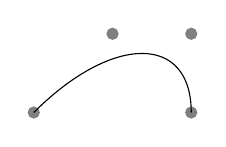
\begin{tikzpicture}
  \filldraw [gray] (0,0) circle [radius=2pt]
                   (1,1) circle [radius=2pt]
                   (2,1) circle [radius=2pt]
                   (2,0) circle [radius=2pt];
  \draw (0,0) .. controls (1,1) and (2,1) .. (2,0);
\end{tikzpicture}
\end{codeexample}

The general syntax for extending a path in a ``curved'' way is
|.. controls| \meta{first control point} |and| \meta{second control
  point} |..| \meta{end point}. You can leave out the |and|
\meta{second control point}, which causes the first one to be used
twice.

So, Karl can now add the first half circle to the picture:

\begin{codeexample}[]
\begin{tikzpicture}
  \draw (-1.5,0) -- (1.5,0);
  \draw (0,-1.5) -- (0,1.5);
  \draw (-1,0) .. controls (-1,0.555) and (-0.555,1) .. (0,1)
               .. controls (0.555,1) and (1,0.555) .. (1,0);
\end{tikzpicture}
\end{codeexample}

Karl is happy with the result, but finds specifying circles in this
way to be extremely awkward. Fortunately, there is a much simpler way.


\subsection{Circle Path Construction}

In order to draw a circle, the path construction operation |circle| can
be used. This operation is followed by a radius in brackets as in
the following example: (Note that the previous position is used as the
\emph{center} of the circle.)

\begin{codeexample}[]
\tikz \draw (0,0) circle [radius=10pt];
\end{codeexample}

You can also append an ellipse to the path using the |ellipse|
operation. Instead of a single radius you can specify two of them:

\begin{codeexample}[]
\tikz \draw (0,0) ellipse [x radius=20pt, y radius=10pt];
\end{codeexample}

To draw an ellipse whose axes are not horizontal and vertical, but
point in an arbitrary direction (a ``turned ellipse'' like \tikz
\draw[rotate=30] (0,0) ellipse [x radius=6pt, y radius=3pt];) you can use
transformations, which are explained later. The code for the little
ellipse is |\tikz \draw[rotate=30] (0,0) ellipse [x radius=6pt, y radius=3pt];|, by
the way.

So, returning to Karl's problem, he can write
|\draw (0,0) circle [radius=1cm];| to draw the circle:

\begin{codeexample}[]
\begin{tikzpicture}
  \draw (-1.5,0) -- (1.5,0);
  \draw (0,-1.5) -- (0,1.5);
  \draw (0,0) circle [radius=1cm];
\end{tikzpicture}
\end{codeexample}


At this point, Karl is a bit alarmed that the circle is so small when
he wants the final picture to be much bigger. He is pleased to learn
that \tikzname\ has powerful transformation options and scaling
everything by a factor of three is very easy. But let us leave the
size as it is for the moment to save some space.




\subsection{Rectangle Path Construction}

The next things we would like to have is the grid in the background.
There are several ways to produce it. For example, one might draw lots of
rectangles. Since rectangles are so common, there is a special syntax
for them: To add a rectangle to the current path, use the |rectangle|
path construction operation. This operation should be followed by another
coordinate and will append a rectangle to the path such that the
previous coordinate and the next coordinates are corners of the
rectangle. So, let us add two rectangles to the picture:

\begin{codeexample}[]
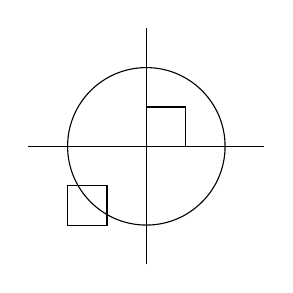
\begin{tikzpicture}
  \draw (-1.5,0) -- (1.5,0);
  \draw (0,-1.5) -- (0,1.5);
  \draw (0,0) circle [radius=1cm];
  \draw (0,0) rectangle (0.5,0.5);
  \draw (-0.5,-0.5) rectangle (-1,-1);
\end{tikzpicture}
\end{codeexample}

While this may be nice in other situations, this is not really leading
anywhere with Karl's problem: First, we would need an awful lot of
these rectangles and then there is the border that is not ``closed.''

So, Karl is about to resort to simply drawing four vertical and four
horizontal lines using the nice |\draw| command, when he learns that
there is a |grid| path construction operation.



\subsection{Grid Path Construction}

The |grid| path operation adds a grid to the current path. It will add
lines making up a grid that fills the rectangle whose one corner is
the current point and whose other corner is the point following the
|grid| operation. For example, the code
|\tikz \draw[step=2pt] (0,0) grid (10pt,10pt);| produces \tikz
\draw[step=2pt] (0,0) grid (10pt,10pt);. Note how the optional
argument for |\draw| can be used to specify a grid width (there are
also |xstep| and |ystep| to define the steppings independently). As
Karl will learn soon, there are \emph{lots} of things that can be
influenced using such options.

For Karl, the following code could be used:

\begin{codeexample}[]
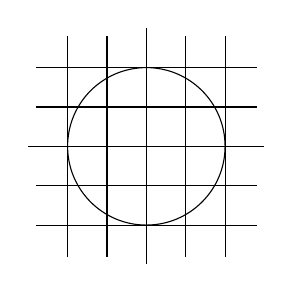
\begin{tikzpicture}
  \draw (-1.5,0) -- (1.5,0);
  \draw (0,-1.5) -- (0,1.5);
  \draw (0,0) circle [radius=1cm];
  \draw[step=.5cm] (-1.4,-1.4) grid (1.4,1.4);
\end{tikzpicture}
\end{codeexample}

Having another look at the desired picture, Karl notices that it would
be nice for the grid to be more subdued. (His son told him that grids
tend to be distracting if they are not subdued.) To subdue the grid,
Karl adds two more options to the |\draw| command that draws the
grid. First, he uses the color |gray| for the grid lines. Second, he
reduces the line width to |very thin|. Finally, he swaps the ordering
of the commands so that the grid is drawn first and everything else on
top.

\begin{codeexample}[]
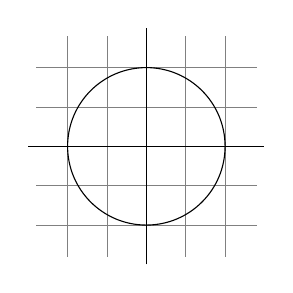
\begin{tikzpicture}
  \draw[step=.5cm,gray,very thin] (-1.4,-1.4) grid (1.4,1.4);
  \draw (-1.5,0) -- (1.5,0);
  \draw (0,-1.5) -- (0,1.5);
  \draw (0,0) circle [radius=1cm];
\end{tikzpicture}
\end{codeexample}


\subsection{Adding a Touch of  Style}

Instead of the options |gray,very thin| Karl could also have
said |help lines|. \emph{Styles} are predefined sets of options
that can be used to organize how a graphic is drawn. By saying
|help lines| you say ``use the style that I (or someone else)
has set for drawing help lines.'' If Karl decides, at some later
point, that grids should be drawn, say, using the color |blue!50|
instead of |gray|, he could provide the following option somewhere:
\begin{codeexample}[code only]
help lines/.style={color=blue!50,very thin}
\end{codeexample}
The effect of this ``style setter'' is that in the current
scope or environment the |help lines| option has the same effect as
|color=blue!50,very thin|.

Using styles makes your graphics code more flexible. You can
change the way things look easily in a consistent manner.
Normally, styles are defined at the beginning of a picture. However,
you may sometimes wish to define a style globally, so that all
pictures of your document can use this style. Then you can easily
change the way all graphics look by changing this one style. In this
situation you can use the |\tikzset| command at the beginning of the
document as in
\begin{codeexample}[code only]
\tikzset{help lines/.style=very thin}
\end{codeexample}

To build a hierarchy of styles you can have one style use
another. So in order to define a style |Karl's grid| that is based on
the |grid| style Karl could say
\begin{codeexample}[code only]
\tikzset{Karl's grid/.style={help lines,color=blue!50}}
...
\draw[Karl's grid] (0,0) grid (5,5);
\end{codeexample}

Styles are made even more powerful by parametrization. This means
that, like other options, styles can also be used with a
parameter. For instance, Karl could parameterize his grid so that, by
default, it is blue, but he could also use another color.

\begin{codeexample}[code only]
\begin{tikzpicture}
  [Karl's grid/.style  ={help lines,color=#1!50},
   Karl's grid/.default=blue]

  \draw[Karl's grid]     (0,0) grid (1.5,2);
  \draw[Karl's grid=red] (2,0) grid (3.5,2);
\end{tikzpicture}
\end{codeexample}


\subsection{Drawing Options}

Karl wonders what other options there are that influence how a path is
drawn. He saw already that the |color=|\meta{color} option can be used
to set the line's color. The option |draw=|\meta{color} does nearly
the same, only it sets the color for the lines only and a different
color can be used for filling (Karl will need this when he fills the
arc for the angle).

He saw that the style |very thin| yields very thin lines. Karl is not
really surprised by this and neither is he surprised to learn that |thin|
yields thin lines,  |thick| yields thick lines, |very thick| yields
very thick lines, |ultra thick| yields really, really thick lines and
|ultra thin| yields lines that are so thin that low-resolution printers
and displays will have trouble showing them. He wonders what gives
lines of ``normal'' thickness. It turns out that |thin| is the correct
choice, since it gives the same thickness as \TeX's |\hrule|
command. Nevertheless, Karl would like to know whether there is 
anything ``in the middle'' between |thin| and |thick|. There is:
|semithick|.

Another useful thing one can do with lines is to dash or dot them. For
this, the two styles |dashed| and |dotted| can be used, yielding
\tikz[baseline] \draw[dashed] (0,.5ex) -- ++(2em,0pt); and
\tikz[baseline] \draw[dotted] (0,.5ex) 
-- ++(2em,0pt);. Both options also exist in a loose and a dense
version, called |loosely dashed|, |densely dashed|, |loosely dotted|,
and |densely dotted|. If he really, really  needs to, Karl can also
define much more complex dashing patterns with the |dash pattern|
option, but his son insists that dashing is to be used with utmost
care and mostly distracts. Karl's son claims that complicated dashing
patterns are evil. Karl's students do not care about dashing patterns.



\subsection{Arc Path Construction}

Our next obstacle is to draw the arc for the angle. For this, the
|arc| path construction operation is useful, which draws part of a
circle or ellipse. This |arc| operation is followed by options in
brackets that specify the arc. An example would be \texttt{arc[start
  angle=10, end angle=80, radius=10pt]}, which means exactly what it
says. Karl obviously
needs an arc from $0^\circ$ to $30^\circ$. The radius should be
something relatively small, perhaps around one third of the circle's
radius. When one uses the arc path construction operation, the
specified arc will be added with its starting point at the current
position. So, we first have to ``get there.''

\begin{codeexample}[]
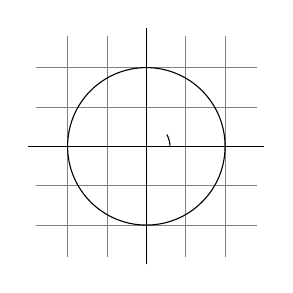
\begin{tikzpicture}
  \draw[step=.5cm,gray,very thin] (-1.4,-1.4) grid (1.4,1.4);
  \draw (-1.5,0) -- (1.5,0);
  \draw (0,-1.5) -- (0,1.5);
  \draw (0,0) circle [radius=1cm];
  \draw (3mm,0mm) arc [start angle=0, end angle=30, radius=3mm];
\end{tikzpicture}
\end{codeexample}

Karl thinks this is really a bit small and he cannot continue unless
he learns how to do scaling. For this, he can add the |[scale=3]|
option. He could add this option to each |\draw| command, but that
would be awkward. Instead, he adds it to the whole environment, which
causes this option to apply to everything within.

\begin{codeexample}[]
\begin{tikzpicture}[scale=3]
  \draw[step=.5cm,gray,very thin] (-1.4,-1.4) grid (1.4,1.4);
  \draw (-1.5,0) -- (1.5,0);
  \draw (0,-1.5) -- (0,1.5);
  \draw (0,0) circle [radius=1cm];
  \draw (3mm,0mm) arc [start angle=0, end angle=30, radius=3mm];
\end{tikzpicture}
\end{codeexample}

As for circles, you can specify ``two'' radii in order to get an
elliptical arc.

\begin{codeexample}[]
  \tikz \draw (0,0) 
    arc [start angle=0, end angle=315, 
         x radius=1.75cm, y radius=1cm];
\end{codeexample}


\subsection{Clipping a Path}

In order to save space in this manual, it would be nice to clip Karl's
graphics a bit so that we can focus on the ``interesting''
parts. Clipping is pretty easy in \tikzname. You can use the |\clip|
command to clip all subsequent drawing. It works like |\draw|, only it
does not draw anything, but uses the given path to clip everything
subsequently.

\begin{codeexample}[]
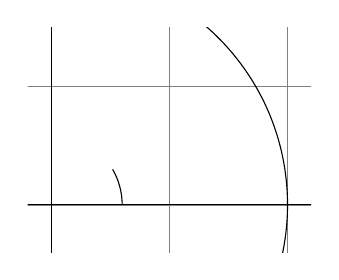
\begin{tikzpicture}[scale=3]
  \clip (-0.1,-0.2) rectangle (1.1,0.75);
  \draw[step=.5cm,gray,very thin] (-1.4,-1.4) grid (1.4,1.4);
  \draw (-1.5,0) -- (1.5,0);
  \draw (0,-1.5) -- (0,1.5);
  \draw (0,0) circle [radius=1cm];
  \draw (3mm,0mm) arc [start angle=0, end angle=30, radius=3mm];
\end{tikzpicture}
\end{codeexample}

You can also do both at the same time: Draw \emph{and} clip a
path. For this, use the |\draw| command and add the |clip|
option. (This is not the whole picture: You can also use the |\clip|
command and add the |draw| option. Well, that is also not the whole
picture: In reality, |\draw| is just a shorthand for |\path[draw]|
and |\clip| is a shorthand for |\path[clip]| and you could also say
|\path[draw,clip]|.) Here is an example:

\begin{codeexample}[]
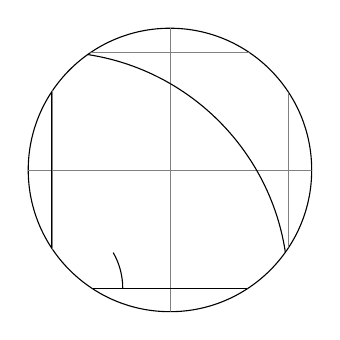
\begin{tikzpicture}[scale=3]
  \clip[draw] (0.5,0.5) circle (.6cm);
  \draw[step=.5cm,gray,very thin] (-1.4,-1.4) grid (1.4,1.4);
  \draw (-1.5,0) -- (1.5,0);
  \draw (0,-1.5) -- (0,1.5);
  \draw (0,0) circle [radius=1cm];
  \draw (3mm,0mm) arc [start angle=0, end angle=30, radius=3mm];
\end{tikzpicture}
\end{codeexample}


\subsection{Parabola and Sine Path Construction}

Although Karl does not need them for his picture, he is pleased to
learn that there are |parabola| and |sin| and |cos| path operations for
adding parabolas and sine and cosine curves to the current path. For the
|parabola| operation, the current point will lie on the parabola as
well as the point given after the parabola operation. Consider
the following example:

\begin{codeexample}[]
\tikz \draw (0,0) rectangle (1,1)  (0,0) parabola (1,1);
\end{codeexample}

It is also possible to place the bend somewhere else:

\begin{codeexample}[]
\tikz \draw[x=1pt,y=1pt] (0,0) parabola bend (4,16) (6,12);
\end{codeexample}

The operations |sin| and |cos| add a sine or cosine curve in the interval
$[0,\pi/2]$ such that the previous current point is at the start of
the curve and the curve ends at the given end point. Here are two
examples:
\begin{codeexample}[]
A sine \tikz \draw[x=1ex,y=1ex] (0,0) sin (1.57,1); curve.
\end{codeexample}

\begin{codeexample}[]
\tikz \draw[x=1.57ex,y=1ex] (0,0) sin (1,1) cos (2,0) sin (3,-1) cos (4,0)
                            (0,1) cos (1,0) sin (2,-1) cos (3,0) sin (4,1);
\end{codeexample}



\subsection{Filling and Drawing}

Returning to the picture, Karl now wants the angle to be ``filled''
with a very light green. For this he uses |\fill| instead of
|\draw|. Here is what Karl does:

\begin{codeexample}[]
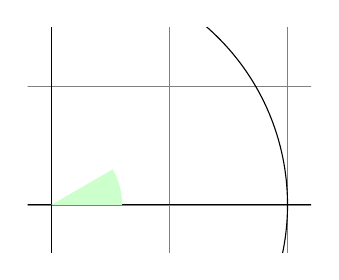
\begin{tikzpicture}[scale=3]
  \clip (-0.1,-0.2) rectangle (1.1,0.75);
  \draw[step=.5cm,gray,very thin] (-1.4,-1.4) grid (1.4,1.4);
  \draw (-1.5,0) -- (1.5,0);
  \draw (0,-1.5) -- (0,1.5);
  \draw (0,0) circle [radius=1cm];
  \fill[green!20!white] (0,0) -- (3mm,0mm)
    arc [start angle=0, end angle=30, radius=3mm] -- (0,0);
\end{tikzpicture}
\end{codeexample}

The color |green!20!white| means 20\% green and 80\% white mixed
together. Such color expression are possible since \tikzname\ uses Uwe
Kern's |xcolor| package, see the documentation of that package for
details on color expressions.

What would have happened, if Karl had not ``closed'' the path using
|--(0,0)| at the end? In this case, the path is closed automatically,
so this could have been omitted. Indeed, it would even have been
better to write the following, instead:
\begin{codeexample}[code only]
  \fill[green!20!white] (0,0) -- (3mm,0mm)
    arc [start angle=0, end angle=30, radius=3mm] -- cycle;
\end{codeexample}
The |--cycle| causes the current path to be closed (actually the
current part of the current path) by smoothly joining the first and
last point. To appreciate the difference, consider the following
example:

\begin{codeexample}[]
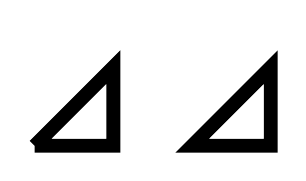
\begin{tikzpicture}[line width=5pt]
  \draw (0,0) -- (1,0) -- (1,1) -- (0,0);
  \draw (2,0) -- (3,0) -- (3,1) -- cycle;
  \useasboundingbox (0,1.5); % make bounding box higher
\end{tikzpicture}
\end{codeexample}

You can also fill and draw a path at the same time using the
|\filldraw| command. This will first draw the path, then fill it. This
may not seem too useful, but you can specify different colors to be
used for filling and for stroking. These are specified as optional
arguments like this:

\begin{codeexample}[]
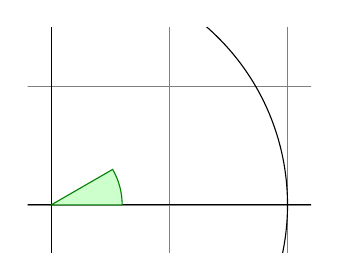
\begin{tikzpicture}[scale=3]
  \clip (-0.1,-0.2) rectangle (1.1,0.75);
  \draw[step=.5cm,gray,very thin] (-1.4,-1.4) grid (1.4,1.4);
  \draw (-1.5,0) -- (1.5,0);
  \draw (0,-1.5) -- (0,1.5);
  \draw (0,0) circle [radius=1cm];
  \filldraw[fill=green!20!white, draw=green!50!black] (0,0) -- (3mm,0mm)
    arc [start angle=0, end angle=30, radius=3mm] -- cycle;
\end{tikzpicture}
\end{codeexample}



\subsection{Shading}

Karl briefly considers the possibility of making the angle ``more
fancy'' by \emph{shading} it. Instead of filling the area with a uniform
color, a smooth transition between different colors is used. For this,
|\shade| and |\shadedraw|, for shading and drawing at the same time,
can be used:

\begin{codeexample}[]
  \tikz \shade (0,0) rectangle (2,1)  (3,0.5) circle (.5cm);
\end{codeexample}
The default shading is a smooth transition from gray to white. To
specify different colors, you can use options:

\begin{codeexample}[]

\begin{tikzpicture}[rounded corners,ultra thick]
  \shade[top color=yellow,bottom color=black] (0,0) rectangle +(2,1);
  \shade[left color=yellow,right color=black] (3,0) rectangle +(2,1);
  \shadedraw[inner color=yellow,outer color=black,draw=yellow] (6,0) rectangle +(2,1);
  \shade[ball color=green] (9,.5) circle (.5cm);
\end{tikzpicture}
\end{codeexample}

For Karl, the following might be appropriate:

\begin{codeexample}[]
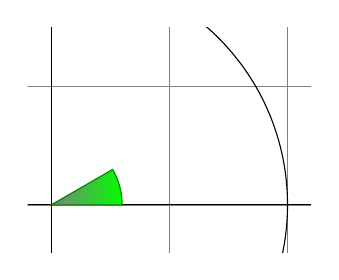
\begin{tikzpicture}[scale=3]
  \clip (-0.1,-0.2) rectangle (1.1,0.75);
  \draw[step=.5cm,gray,very thin] (-1.4,-1.4) grid (1.4,1.4);
  \draw (-1.5,0) -- (1.5,0);
  \draw (0,-1.5) -- (0,1.5);
  \draw (0,0) circle [radius=1cm];
  \shadedraw[left color=gray,right color=green, draw=green!50!black]
    (0,0) -- (3mm,0mm)
    arc [start angle=0, end angle=30, radius=3mm] -- cycle;
\end{tikzpicture}
\end{codeexample}

However, he wisely decides that shadings usually only distract without
adding anything to the picture.


\subsection{Specifying Coordinates}

Karl now wants to add the sine and cosine lines. He knows already that
he can use the |color=| option to set the lines' colors. So, what is
the best way to specify the coordinates?

There are different ways of specifying coordinates. The easiest way is
to say something like |(10pt,2cm)|. This means 10pt in $x$-direction
and 2cm in $y$-directions. Alternatively, you can also leave out the
units as in |(1,2)|, which means ``one times the current $x$-vector
plus twice the current $y$-vector.'' These vectors default to 1cm in
the $x$-direction and 1cm in the $y$-direction, respectively.

In order to specify points in polar coordinates, use the notation
|(30:1cm)|, which means 1cm in direction 30 degree. This is obviously
quite useful to ``get to the point $(\cos 30^\circ,\sin 30^\circ)$ on
the circle.''

You can add a single |+| sign in front of a coordinate or two of
them as in |+(0cm,1cm)| or |++(2cm,0cm)|. Such coordinates are interpreted
differently: The first form means ``1cm upwards from the previous
specified position'' and the second means ``2cm to the right of the
previous specified position, making this the new specified position.''
For example, we can draw the sine line as follows:

\begin{codeexample}[]
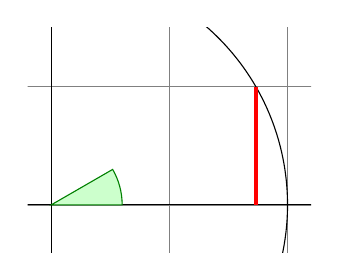
\begin{tikzpicture}[scale=3]
  \clip (-0.1,-0.2) rectangle (1.1,0.75);
  \draw[step=.5cm,gray,very thin] (-1.4,-1.4) grid (1.4,1.4);
  \draw (-1.5,0) -- (1.5,0);
  \draw (0,-1.5) -- (0,1.5);
  \draw (0,0) circle [radius=1cm];
  \filldraw[fill=green!20,draw=green!50!black] (0,0) -- (3mm,0mm)
      arc [start angle=0, end angle=30, radius=3mm] -- cycle;
  \draw[red,very thick] (30:1cm) -- +(0,-0.5);
\end{tikzpicture}
\end{codeexample}

Karl used the fact $\sin 30^\circ = 1/2$. However, he very much
doubts that his students know this, so it would be nice to have a way
of specifying ``the point straight down from |(30:1cm)| that lies on
the $x$-axis.'' This is, indeed, possible using a special syntax: Karl
can write \verb!(30:1cm |- 0,0)!. In general, the meaning of
|(|\meta{p}\verb! |- !\meta{q}|)| is ``the intersection of a vertical
line through $p$ and a horizontal line through $q$.''

Next, let us draw the cosine line. One way would be to say
\verb!(30:1cm |- 0,0) -- (0,0)!. Another way is the following: we
``continue'' from where the sine ends:

\begin{codeexample}[]
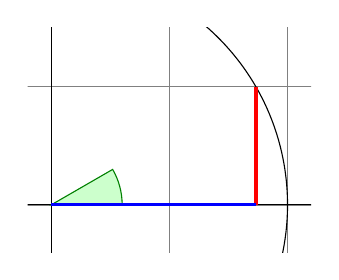
\begin{tikzpicture}[scale=3]
  \clip (-0.1,-0.2) rectangle (1.1,0.75);
  \draw[step=.5cm,gray,very thin] (-1.4,-1.4) grid (1.4,1.4);
  \draw (-1.5,0) -- (1.5,0);
  \draw (0,-1.5) -- (0,1.5);
  \draw (0,0) circle [radius=1cm];
  \filldraw[fill=green!20,draw=green!50!black] (0,0) -- (3mm,0mm)
      arc [start angle=0, end angle=30, radius=3mm] -- cycle;
  \draw[red,very thick]  (30:1cm) -- +(0,-0.5);
  \draw[blue,very thick] (30:1cm) ++(0,-0.5) -- (0,0);
\end{tikzpicture}
\end{codeexample}

Note that there is no |--| between |(30:1cm)| and |++(0,-0.5)|. In
detail, this path is interpreted as follows: ``First, the |(30:1cm)|
tells me to move by pen to $(\cos 30^\circ,1/2)$. Next, there comes
another coordinate specification, so I move my pen there without drawing
anything. This new point is half a unit down from the last position,
thus it is at $(\cos 30^\circ,0)$. Finally, I move the pen to the
origin, but this time drawing something (because of the |--|).''

To appreciate the difference between |+| and |++| consider the
following example:

\begin{codeexample}[]
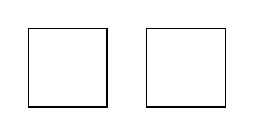
\begin{tikzpicture}
  \def\rectanglepath{-- ++(1cm,0cm)  -- ++(0cm,1cm)  -- ++(-1cm,0cm) -- cycle}
  \draw (0,0) \rectanglepath;
  \draw (1.5,0) \rectanglepath;
\end{tikzpicture}
\end{codeexample}

By comparison, when using a single |+|, the coordinates are different:

\begin{codeexample}[]
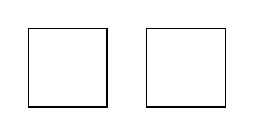
\begin{tikzpicture}
  \def\rectanglepath{-- +(1cm,0cm)  -- +(1cm,1cm)  -- +(0cm,1cm) -- cycle}
  \draw (0,0) \rectanglepath;
  \draw (1.5,0) \rectanglepath;
\end{tikzpicture}
\end{codeexample}


Naturally, all of this could have been written more clearly and more
economically like this (either with a single of a double |+|):
\begin{codeexample}[]
\tikz \draw (0,0) rectangle +(1,1)  (1.5,0) rectangle +(1,1);
\end{codeexample}


\subsection{Intersecting Paths}

Karl is left with the line for $\tan \alpha$, which seems difficult to
specify using transformations and polar coordinates. The first -- and
easiest -- thing he can do is so simply use the coordinate
|(1,{tan(30)})| since \tikzname's math engine knows how to compute
things like |tan(30)|. Note the added braces since, otherwise,
\tikzname's parser would think that the first closing parenthesis ends
the coordinate (in general, you need to add braces around components
of coordinates when these components contain parentheses). 

Karl can, however, also use a more elaborate, but also more
``geometric'' way of computing the length of the orange line: He can
specify intersections of paths as coordinates. The line for $\tan
\alpha$ starts at $(1,0)$ 
and goes upward to a point that is at the intersection of a line going
``up'' and a line going from the origin through |(30:1cm)|. Such
computations are made available by the |intersections| library.

What Karl must do is to create two ``invisible'' paths that intersect
at the position of interest. Creating paths that are not otherwise
seen can be done using the |\path| command without any options like
|draw| or |fill|. Then, Karl can add the |name path| option to the
path for later reference. Once the paths have been constructed, Karl
can use the |name intersections| to assign names to the coordinate for
later reference.

\begin{codeexample}[code only]
\path [name path=upward line] (1,0) -- (1,1);
\path [name path=sloped line] (0,0) -- (30:1.5cm); % a bit longer, so that there is an intersection

\draw [name intersections={of=upward line and sloped line, by=x}]
  [very thick,orange] (1,0) -- (x);
\end{codeexample}


\subsection{Adding Arrow Tips}

Karl now wants to add the little arrow tips at the end of the axes. He has
noticed that in many plots, even in scientific journals, these arrow tips
seem to be missing, presumably because the generating programs cannot
produce them. Karl thinks arrow tips belong at the end of axes. His
son agrees. His students do not care about arrow tips.

It turns out that adding arrow tips is pretty easy: Karl adds the option
|->| to the drawing commands for the axes:

\begin{codeexample}[]
\begin{tikzpicture}[scale=3]
  \clip (-0.1,-0.2) rectangle (1.1,1.51);
  \draw[step=.5cm,gray,very thin] (-1.4,-1.4) grid (1.4,1.4);
  \draw[->] (-1.5,0) -- (1.5,0);
  \draw[->] (0,-1.5) -- (0,1.5);
  \draw (0,0) circle [radius=1cm];
  \filldraw[fill=green!20,draw=green!50!black] (0,0) -- (3mm,0mm)
        arc [start angle=0, end angle=30, radius=3mm] -- cycle;
  \draw[red,very thick]    (30:1cm) -- +(0,-0.5);
  \draw[blue,very thick]   (30:1cm) ++(0,-0.5) -- (0,0);

  \path [name path=upward line] (1,0) -- (1,1);
  \path [name path=sloped line] (0,0) -- (30:1.5cm);
  \draw [name intersections={of=upward line and sloped line, by=x}]
        [very thick,orange] (1,0) -- (x);
\end{tikzpicture}
\end{codeexample}

If Karl had used the option |<-| instead of |->|, arrow tips would
have been put at the beginning of the path. The option |<->| puts
arrow tips at both ends of the path.

There are certain restrictions to the kind of paths to which arrow tips
can be added. As a rule of thumb, you can add arrow tips only to a
single open ``line.'' For example, you cannot add tips to,
say, a rectangle or a circle. However, you can add arrow
tips to curved paths and to paths that have several segments, as in
the following examples:

\begin{codeexample}[]
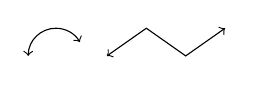
\begin{tikzpicture}
  \draw [<->] (0,0) arc [start angle=180, end angle=30, radius=10pt];
  \draw [<->] (1,0) -- (1.5cm,10pt) -- (2cm,0pt) -- (2.5cm,10pt);
\end{tikzpicture}
\end{codeexample}

Karl has a more detailed look at the arrow that \tikzname\ puts at the
end. It looks like this when he zooms it: \tikz[baseline]
\draw[->,line width=1pt] (0pt,.5ex) -- ++(10pt,0pt);. The shape seems
vaguely familiar and, indeed, this is exactly the end of \TeX's
standard arrow used in something like $f\colon A \to B$.

Karl likes the arrow, especially since it is not ``as thick'' as the
arrows offered by many other packages. However, he expects that,
sometimes, he might need to use some other kinds of arrow.
To do so, Karl can say |>=|\meta{kind of end arrow tip}, where
\meta{kind of end arrow tip} is a special arrow tip specification. For
example, if Karl says |>=Stealth|, then he tells \tikzname\
that he would like  ``stealth-fighter-like'' arrow tips:

\begin{codeexample}[]
\begin{tikzpicture}[>=Stealth]
  \draw [->] (0,0) arc [start angle=180, end angle=30, radius=10pt];
  \draw [<<-,very thick] (1,0) -- (1.5cm,10pt) -- (2cm,0pt) -- (2.5cm,10pt);
\end{tikzpicture}
\end{codeexample}%>>

Karl wonders whether such a military name for the arrow type is really
necessary. He is not really mollified when his son tells him that
Microsoft's PowerPoint uses the same name. He decides to have his
students discuss this at some point.

In addition to |Stealth| there are several other predefined kinds of
arrow tips Karl can choose from, see Section~\ref{section-arrows}. Furthermore,
he can define arrows types himself, if he needs new ones.


\subsection{Scoping}

Karl saw already that there are numerous graphic options that affect how
paths are rendered. Often, he would like to apply certain options to
a whole set of graphic commands. For example, Karl might wish to draw
three paths using a |thick| pen, but would like everything else to
be drawn ``normally.''

If Karl wishes to set a certain graphic option for the whole picture,
he can simply pass this option to the |\tikz| command or to the
|{tikzpicture}| environment (Gerda would pass the options to
|\tikzpicture| and Hans passes them to |\starttikzpicture|). However,
if Karl wants to apply graphic options to a local group, he put these
commands inside a |{scope}| environment (Gerda uses |\scope| and
|\endscope|, Hans uses |\startscope| and |\stopscope|). This
environment takes graphic options as an optional argument and these
options apply to everything inside the scope, but not to anything outside.

Here is an example:

\begin{codeexample}[]
\begin{tikzpicture}[ultra thick]
  \draw (0,0) -- (0,1);
  \begin{scope}[thin]
    \draw (1,0) -- (1,1);
    \draw (2,0) -- (2,1);
  \end{scope}
  \draw (3,0) -- (3,1);
\end{tikzpicture}
\end{codeexample}

Scoping has another interesting effect: Any changes to the clipping
area are local to the scope. Thus, if you say |\clip| somewhere inside
a scope, the effect of the |\clip| command ends at the end of the
scope. This is useful since there is no other way of ``enlarging'' the
clipping area.

Karl has also already seen that giving options to commands like
|\draw| apply only to that command. It turns out that the situation is
slightly more complex. First, options to a command like |\draw| are
not really options to the command, but they are ``path options'' and
can be given anywhere on the path. So, instead of
|\draw[thin] (0,0) -- (1,0);| one can also write
|\draw (0,0) [thin] -- (1,0);| or |\draw (0,0) -- (1,0) [thin];|; all
of these have the same effect. This might seem strange since in the
last case, it would appear that the |thin| should take effect only
``after'' the line from $(0,0)$ to $(1,0)$ has been drawn. However,
most graphic options only apply to the whole path. Indeed, if you say
both |thin| and |thick| on the same path, the last option given will
``win.''

When reading the above, Karl notices that only ``most'' graphic
options apply to the whole path. Indeed, all transformation options do
\emph{not} apply to the whole path, but only to ``everything following
them on the path.'' We will have a more detailed look at this in a
moment. Nevertheless, all options given during a path construction
apply only to this path.



\subsection{Transformations}

When you specify a  coordinate like |(1cm,1cm)|, where is that
coordinate placed on the page? To determine the position, \tikzname,
\TeX, and \textsc{pdf} or PostScript all apply certain transformations
to the given coordinate in order to determine the final position on
the page.

\tikzname\ provides numerous options that allow you to transform
coordinates in \tikzname's private coordinate system. For example, the
|xshift| option allows you to shift all subsequent points by a certain
amount:

\begin{codeexample}[]
\tikz \draw (0,0) -- (0,0.5) [xshift=2pt] (0,0) -- (0,0.5);
\end{codeexample}

It is important to note that you can change transformation ``in the
middle of a path,'' a feature that is not supported by \pdf\
or PostScript. The reason is that \tikzname\ keeps track of its own
transformation matrix.

Here is a more complicated example:
\begin{codeexample}[]
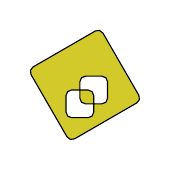
\begin{tikzpicture}[even odd rule,rounded corners=2pt,x=10pt,y=10pt]
  \filldraw[fill=yellow!80!black] (0,0)   rectangle (1,1)
        [xshift=5pt,yshift=5pt]   (0,0)   rectangle (1,1)
                    [rotate=30]   (-1,-1) rectangle (2,2);
\end{tikzpicture}
\end{codeexample}

The most useful transformations are |xshift| and |yshift| for
shifting, |shift| for shifting to a given point as in |shift={(1,0)}|
or |shift={+(0,0)}| (the braces are necessary so that \TeX\ does not
mistake the comma for separating options), |rotate| for rotating by a
certain angle (there is also a |rotate around| for rotating around a
given point), |scale| for scaling by a certain factor, |xscale| and
|yscale| for scaling only in the $x$- or $y$-direction (|xscale=-1| is
a flip), and |xslant| and |yslant| for slanting. If these
transformation and those that I have not mentioned are not
sufficient,  the |cm| option allows you to apply an arbitrary
transformation matrix. Karl's students, by the way, do not know what a
transformation matrix is.



\subsection{Repeating Things: For-Loops}

Karl's next aim is to add little ticks on the axes at positions $-1$,
$-1/2$, $1/2$, and $1$. For this, it would be nice to use some kind of
``loop,'' especially since he wishes to do the same thing at each of
these positions. There are different packages for doing this. \LaTeX\
has its own internal command for this, |pstricks| comes along with the
powerful |\multido| command. All of these can be used together with
\tikzname, so if you are familiar with them, feel free to
use them. \tikzname\ introduces yet another command, called |\foreach|,
which I introduced since I could never remember the syntax of the other
packages. |\foreach| is defined in the package |pgffor| and can be used
independently \tikzname, but \tikzname\ includes it automatically.

In its basic form, the |\foreach| command is easy to use:
\begin{codeexample}[]
\foreach \x in {1,2,3} {$x =\x$, }
\end{codeexample}

The general syntax is |\foreach| \meta{variable}| in {|\meta{list of
    values}|} |\meta{commands}. Inside the \meta{commands}, the
\meta{variable} will be assigned to the different values. If the
\meta{commands} do not start with a brace, everything up to the
next semicolon is used as \meta{commands}.

For Karl and the ticks on the axes, he could use the following code:

\begin{codeexample}[]
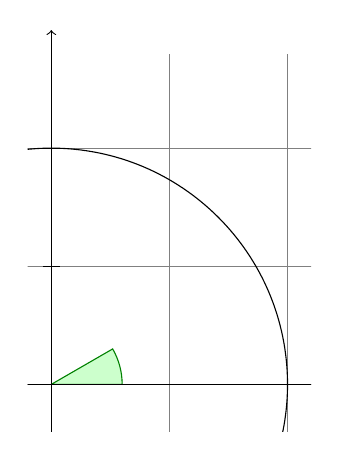
\begin{tikzpicture}[scale=3]
  \clip (-0.1,-0.2) rectangle (1.1,1.51);
  \draw[step=.5cm,gray,very thin] (-1.4,-1.4) grid (1.4,1.4);
  \filldraw[fill=green!20,draw=green!50!black] (0,0) -- (3mm,0mm)
      arc [start angle=0, end angle=30, radius=3mm] -- cycle;
  \draw[->] (-1.5,0) -- (1.5,0);
  \draw[->] (0,-1.5) -- (0,1.5);
  \draw (0,0) circle [radius=1cm];

  \foreach \x in {-1cm,-0.5cm,1cm}
    \draw (\x,-1pt) -- (\x,1pt);
  \foreach \y in {-1cm,-0.5cm,0.5cm,1cm}
    \draw (-1pt,\y) -- (1pt,\y);
\end{tikzpicture}
\end{codeexample}

As a matter of fact, there are many different ways of creating the
ticks. For example, Karl could have put the |\draw ...;| inside curly
braces. He could also have used, say,
\begin{codeexample}[code only]
\foreach \x in {-1,-0.5,1}
  \draw[xshift=\x cm] (0pt,-1pt) -- (0pt,1pt);
\end{codeexample}

Karl is curious what would happen in a more complicated situation
where there are, say, 20 ticks. It seems bothersome to explicitly
mention all these numbers in the set for |\foreach|. Indeed, it is
possible to use |...| inside the |\foreach| statement to iterate over
a large number of values (which must, however, be dimensionless
real numbers) as in the following example:

\begin{codeexample}[]
\tikz \foreach \x in {1,...,10}
        \draw (\x,0) circle (0.4cm);
\end{codeexample}

If you provide \emph{two} numbers before the |...|, the |\foreach|
statement will use their difference for the stepping:

\begin{codeexample}[]
\tikz \foreach \x in {-1,-0.5,...,1}
       \draw (\x cm,-1pt) -- (\x cm,1pt);
\end{codeexample}

We can also nest loops to create interesting effects:

\begin{codeexample}[]
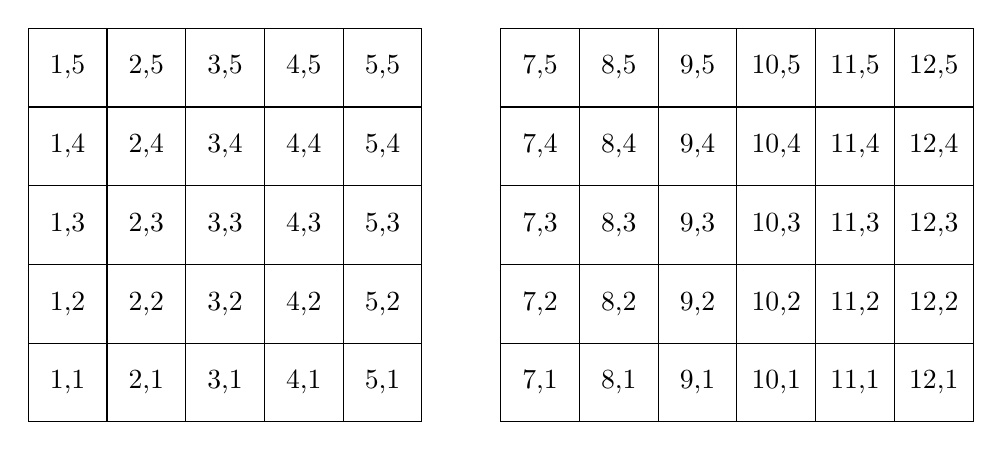
\begin{tikzpicture}
  \foreach \x in {1,2,...,5,7,8,...,12}
    \foreach \y in {1,...,5}
    {
      \draw (\x,\y) +(-.5,-.5) rectangle ++(.5,.5);
      \draw (\x,\y) node{\x,\y};
    }
\end{tikzpicture}
\end{codeexample}

The |\foreach| statement can do even trickier stuff, but the above
gives the idea.




\subsection{Adding Text}

Karl is, by now, quite satisfied with the picture. However, the most
important parts, namely the labels, are still missing!

\tikzname\ offers an easy-to-use and powerful system for adding text and,
more generally, complex shapes to a picture at specific positions. The
basic idea is the following: When \tikzname\ is constructing a path and
encounters the keyword |node| in the middle of a path, it
reads a \emph{node specification}. The keyword |node| is typically
followed by some options and then some text between curly braces. This
text is put inside a normal \TeX\ box (if the node specification
directly follows a coordinate, which is usually the case, \tikzname\ is
able to perform some magic so that it is even possible to use verbatim
text inside the boxes) and then placed at the current position, that
is, at the last specified position (possibly shifted a bit, according
to the given options). However, all nodes are drawn only after the
path has been completely drawn/filled/shaded/clipped/whatever.

\begin{codeexample}[]
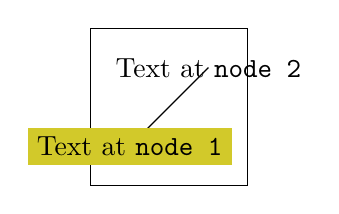
\begin{tikzpicture}
  \draw (0,0) rectangle (2,2);
  \draw (0.5,0.5) node [fill=yellow!80!black]
                       {Text at \verb!node 1!}
     -- (1.5,1.5) node {Text at \verb!node 2!};
\end{tikzpicture}
\end{codeexample}

Obviously, Karl would not only like to place nodes \emph{on} the last
specified position, but also to the left or the
right of these positions. For this, every node object that you
put in your picture is equipped with several \emph{anchors}. For
example, the |north| anchor is in the middle at the upper end of the shape,
the |south| anchor is at the bottom and the |north east| anchor is in
the upper right corner. When you give the option |anchor=north|, the
text will be placed such that this northern anchor will lie on the
current position and the text is, thus, below the current
position. Karl uses this to draw the ticks as follows:

\begin{codeexample}[]
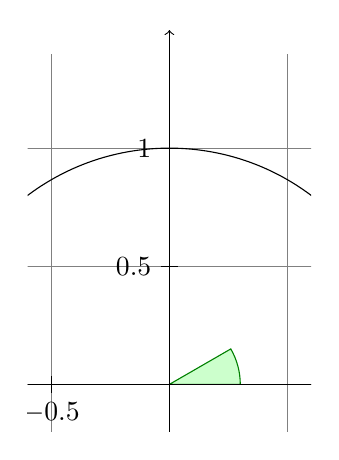
\begin{tikzpicture}[scale=3]
  \clip (-0.6,-0.2) rectangle (0.6,1.51);
  \draw[step=.5cm,help lines] (-1.4,-1.4) grid (1.4,1.4);
  \filldraw[fill=green!20,draw=green!50!black] (0,0) -- (3mm,0mm)
    arc [start angle=0, end angle=30, radius=3mm] -- cycle;
  \draw[->] (-1.5,0) -- (1.5,0);   \draw[->] (0,-1.5) -- (0,1.5);
  \draw (0,0) circle [radius=1cm];

  \foreach \x in {-1,-0.5,1}
    \draw (\x cm,1pt) -- (\x cm,-1pt) node[anchor=north] {$\x$};
  \foreach \y in {-1,-0.5,0.5,1}
    \draw (1pt,\y cm) -- (-1pt,\y cm) node[anchor=east] {$\y$};
\end{tikzpicture}
\end{codeexample}

This is quite nice, already. Using these anchors, Karl can now add
most of the other text elements. However, Karl thinks that, though
``correct,'' it is quite counter-intuitive that in order to place something
\emph{below} a given point, he has to use the \emph{north} anchor. For
this reason, there is an option called |below|, which does the
same as |anchor=north|. Similarly, |above right| does the same as
|anchor=south west|. In addition, |below| takes an optional
dimension argument. If given, the shape will additionally be shifted
downwards by the given amount. So, |below=1pt| can be used to put
a text label below some point and, additionally shift it  1pt
downwards.

Karl is not quite satisfied with the ticks. He would like to have
$1/2$ or $\frac{1}{2}$ shown instead of $0.5$, partly to show off the
nice capabilities of \TeX\ and \tikzname, partly because for positions
like $1/3$ or $\pi$ it is certainly very much preferable to have the
``mathematical'' tick there instead of just the ``numeric'' tick.
His students, on the other hand, prefer $0.5$ over $1/2$
since they are not too fond of fractions in general.

Karl now faces a problem: For the |\foreach| statement, the position
|\x| should still be given as |0.5| since \tikzname\ will not know where
|\frac{1}{2}| is supposed to be. On the other hand, the typeset text
should really be  |\frac{1}{2}|. To solve this problem, |\foreach|
offers a special syntax: Instead of having one variable |\x|, Karl can
specify two (or even more) variables separated by a slash as in
|\x / \xtext|. Then, the elements in the set over which |\foreach|
iterates must also be of the form \meta{first}|/|\meta{second}. In
each iteration, |\x| will be set to \meta{first} and |\xtext| will be
set to \meta{second}. If no \meta{second} is given, the \meta{first}
will be used again. So, here is the new code for the ticks:

\begin{codeexample}[]
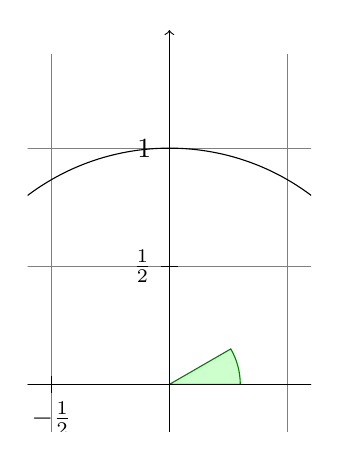
\begin{tikzpicture}[scale=3]
  \clip (-0.6,-0.2) rectangle (0.6,1.51);
  \draw[step=.5cm,help lines] (-1.4,-1.4) grid (1.4,1.4);
  \filldraw[fill=green!20,draw=green!50!black] (0,0) -- (3mm,0mm)
      arc [start angle=0, end angle=30, radius=3mm] -- cycle;
  \draw[->] (-1.5,0) -- (1.5,0); \draw[->] (0,-1.5) -- (0,1.5);
  \draw (0,0) circle [radius=1cm];

  \foreach \x/\xtext in {-1, -0.5/-\frac{1}{2}, 1}
    \draw (\x cm,1pt) -- (\x cm,-1pt) node[anchor=north] {$\xtext$};
  \foreach \y/\ytext in {-1, -0.5/-\frac{1}{2}, 0.5/\frac{1}{2}, 1}
    \draw (1pt,\y cm) -- (-1pt,\y cm) node[anchor=east] {$\ytext$};
\end{tikzpicture}
\end{codeexample}

Karl is quite pleased with the result, but his son points out that
this is still not perfectly satisfactory: The grid and the circle
interfere with the numbers and decrease their legibility. Karl is not
very concerned by this (his students do not even notice), but his son
insists that there is an easy solution: Karl can add the
|[fill=white]| option to fill out the background of the text shape
with a white color.

The next thing Karl wants to do is to add the labels like $\sin
\alpha$. For this, he would like to place a label ``in the middle of
the line.'' To do so, instead of specifying the label
|node {$\sin\alpha$}|  directly after one of the endpoints of the line
(which would place
the label at that endpoint), Karl can give the label directly after
the |--|, before the coordinate. By default, this places the label in
the middle of the line, but the |pos=| options can be used to modify
this. Also, options like |near start| and |near end| can be used to
modify this position:


\begin{codeexample}[]
\begin{tikzpicture}[scale=3]
  \clip (-2,-0.2) rectangle (2,0.8);
  \draw[step=.5cm,gray,very thin] (-1.4,-1.4) grid (1.4,1.4);
  \filldraw[fill=green!20,draw=green!50!black] (0,0) -- (3mm,0mm)
    arc [start angle=0, end angle=30, radius=3mm] -- cycle;
  \draw[->] (-1.5,0) -- (1.5,0) coordinate (x axis);
  \draw[->] (0,-1.5) -- (0,1.5) coordinate (y axis);
  \draw (0,0) circle [radius=1cm];

  \draw[very thick,red]
    (30:1cm) -- node[left=1pt,fill=white] {$\sin \alpha$} (30:1cm |- x axis);
  \draw[very thick,blue]
    (30:1cm |- x axis) -- node[below=2pt,fill=white] {$\cos \alpha$} (0,0);
  \path [name path=upward line] (1,0) -- (1,1);
  \path [name path=sloped line] (0,0) -- (30:1.5cm);
  \draw [name intersections={of=upward line and sloped line, by=t}]
    [very thick,orange] (1,0) -- node [right=1pt,fill=white]
    {$\displaystyle \tan \alpha \color{black}=
      \frac{{\color{red}\sin \alpha}}{\color{blue}\cos \alpha}$} (t);

  \draw (0,0) -- (t);

  \foreach \x/\xtext in {-1, -0.5/-\frac{1}{2}, 1}
    \draw (\x cm,1pt) -- (\x cm,-1pt) node[anchor=north,fill=white] {$\xtext$};
  \foreach \y/\ytext in {-1, -0.5/-\frac{1}{2}, 0.5/\frac{1}{2}, 1}
    \draw (1pt,\y cm) -- (-1pt,\y cm) node[anchor=east,fill=white] {$\ytext$};
\end{tikzpicture}
\end{codeexample}

You can also position labels on curves and, by adding the |sloped|
option, have them rotated such that they match the line's slope. Here
is an example:

\begin{codeexample}[]
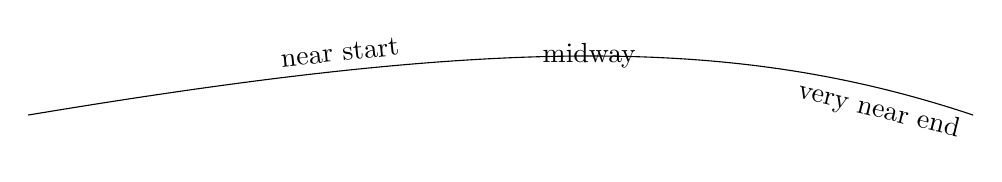
\begin{tikzpicture}
  \draw (0,0) .. controls (6,1) and (9,1) ..
    node[near start,sloped,above] {near start}
    node {midway}
    node[very near end,sloped,below] {very near end} (12,0);
\end{tikzpicture}
\end{codeexample}

It remains to draw the explanatory text at the right of the
picture. The main difficulty here lies in limiting the width of the
text ``label,'' which is quite long, so that line breaking is
used. Fortunately, Karl can use the option |text width=6cm| to get the
desired effect. So, here is the full code:

\begin{codeexample}[code only]
\begin{tikzpicture}
  [scale=3,line cap=round,
  % Styles
  axes/.style=,
  important line/.style={very thick},
  information text/.style={rounded corners,fill=red!10,inner sep=1ex}]

  % Colors
  \colorlet{anglecolor}{green!50!black}
  \colorlet{sincolor}{red}
  \colorlet{tancolor}{orange!80!black}
  \colorlet{coscolor}{blue}

  % The graphic
  \draw[help lines,step=0.5cm] (-1.4,-1.4) grid (1.4,1.4);

  \draw (0,0) circle [radius=1cm];

  \begin{scope}[axes]
    \draw[->] (-1.5,0) -- (1.5,0) node[right] {$x$} coordinate(x axis);
    \draw[->] (0,-1.5) -- (0,1.5) node[above] {$y$} coordinate(y axis);

    \foreach \x/\xtext in {-1, -.5/-\frac{1}{2}, 1}
      \draw[xshift=\x cm] (0pt,1pt) -- (0pt,-1pt) node[below,fill=white] {$\xtext$};

    \foreach \y/\ytext in {-1, -.5/-\frac{1}{2}, .5/\frac{1}{2}, 1}
      \draw[yshift=\y cm] (1pt,0pt) -- (-1pt,0pt) node[left,fill=white] {$\ytext$};
  \end{scope}

  \filldraw[fill=green!20,draw=anglecolor] (0,0) -- (3mm,0pt)
    arc [start angle=0, end angle=30, radius=3mm];
  \draw (15:2mm) node[anglecolor] {$\alpha$};

  \draw[important line,sincolor]
    (30:1cm) -- node[left=1pt,fill=white] {$\sin \alpha$} (30:1cm |- x axis);

  \draw[important line,coscolor]
    (30:1cm |- x axis) -- node[below=2pt,fill=white] {$\cos \alpha$} (0,0);

  \path [name path=upward line] (1,0) -- (1,1);
  \path [name path=sloped line] (0,0) -- (30:1.5cm);
  \draw [name intersections={of=upward line and sloped line, by=t}]
    [very thick,orange] (1,0) -- node [right=1pt,fill=white]
    {$\displaystyle \tan \alpha \color{black}=
      \frac{{\color{red}\sin \alpha}}{\color{blue}\cos \alpha}$} (t);

  \draw (0,0) -- (t);

  \draw[xshift=1.85cm]
    node[right,text width=6cm,information text]
    {
      The {\color{anglecolor} angle $\alpha$} is $30^\circ$ in the
      example ($\pi/6$ in radians). The {\color{sincolor}sine of
        $\alpha$}, which is the height of the red line, is
      \[
      {\color{sincolor} \sin \alpha} = 1/2.
      \]
      By the Theorem of Pythagoras ...
    };
\end{tikzpicture}
\end{codeexample}



\subsection{Pics: The Angle Revisited}

Karl expects that the code of certain parts of the picture he created
might be so useful that he might wish to reuse them in the
future. A natural thing to do is to create \TeX\ macros that store
the code he wishes to reuse. However, \tikzname\ offers another way
that is integrated directly into its parser: pics!

A ``pic'' is ``not quite a full picture,'' hence the short name. The
idea is that a pic is simply some code that you can add to a picture
at different places using the |pic| command whose syntax is almost
identical to the |node| command. The main difference is that instead
of specifying some text in curly braces that should be shown, you
specify the name of a predefined picture that should be shown. 

Defining new pics is easy enough, see Section~\ref{section-pics}, but
right now we just want to use one such predefined pic: the |angle|
pic. As the name suggests, it is a small drawing of an angle
consisting of a little wedge and an arc together with some text (Karl
needs to load the |angle| library and the |quotes| for the following
examples). What makes this pic useful is the fact that the size of the
wedge will be computed automatically.

The |angle| pic draws an angle between the two lines $BA$ and $BC$,
where $A$, $B$, and $C$ are three coordinates. In our case, $B$ is the
origin, $A$ is somewhere on the $x$-axis and $C$ is somewhere on a
line at $30^\circ$. 

\begin{codeexample}[]
\begin{tikzpicture}[scale=3]
  \coordinate (A) at (1,0);
  \coordinate (B) at (0,0);
  \coordinate (C) at (30:1cm);

  \draw (A) -- (B) -- (C)
        pic [draw=green!50!black, fill=green!20, angle radius=9mm,
             "$\alpha$"] {angle = A--B--C};
\end{tikzpicture}  
\end{codeexample}

Let us see, what is happening here. First we have specified three
\emph{coordinates} using the |\coordinate| command. It allows us to
name a specific coordinate in the picture. Then comes something that
starts as a normal |\draw|, but then comes the |pic| command. This
command gets lots of options and, in curly braces, comes the most
important point: We specify that we want to add an |angle| pic and
this angle should be between the points we named |A|, |B|, and |C| (we
could use other names). Note that the text that we want to be shown in
the pic is specified in quotes inside the options of the |pic|, not
inside the curly braces.

To learn more about pics, please see Section~\ref{section-pics}.